%
% 4-fundamental.tex
%
% (c) 2025 Prof Dr Andreas Müller
%
\section{Der Fundamentalsatz der Algebra
\label{buch:komplex:section:fundamental}}
\kopfrechts{Der Fundamentalsatz der Algebra}
Durch Hinzufügen von Nullstellen eines Polynoms kann man einen
Körper so vergrössern, dass das Polynom sich faktorisieren lässt.
Im Prinzip sind dafür für jedes Polynom andere Erweiterungen nötig.
Es stellt sich damit die Frage, ob es vielleicht eine Erweiterung
gibt, in der sich alle Polynome faktorisieren lassen.

%
% 31-nullstellenc.tex -- Nullstellen von Polynomen über C
%
% (c) 2026 Prof Dr Andreas Müller
%
\subsection{Nullstellen von Polynomen über $\mathbb{C}$}
Hat man eine Nullstelle $\alpha$ eines Polynoms $p(X)\in K[X]$ gefunden,
die noch nicht im Koeffizientenkörper enthalten ist, kann man das Polynom
durch $X-\alpha$ dividieren.
Dabei entsteht ein neues Polynom $q(X) = p(X)/(X-\alpha)$,
aber die Koeffizienten dieses neuen Polynoms sind im Allgemeinen nicht
mehr in $K$, sondern in $K(\alpha)$.

\begin{beispiel}
Das Polynom $p(X)=X^2-2\in \mathbb{Q}[X]$ hat die Nullstelle
$\alpha_0=\sqrt[3]{2}$.
Division durch $X-\alpha_0=X-\sqrt[3]{2}$ ergibt ein Polynom vom Grad 2:
\[
\def\p{\phantom{)}}
\def\r{\raisebox{4pt}{\mathstrut}}
\def\m{\llap{$-$}}
\renewcommand{\arraycolsep}{2pt}
\begin{array}{rcrcrcrcrcrcrcrcrcr}
  (X^3 & &                     & &                   &-&             2) &:& (X &-& \!\sqrt[3]{2}) &=& X^2 &+& \!\sqrt[3]{2}X &+& \!\sqrt[3]{4}.\\
\m(X^3 &-&   \!\sqrt[3]{2}X^2) & &                   & &                & &    & &                & &     & &                & &               \\
\cline{1-3}
       & &   \!\sqrt[3]{2}X^2\p& &                   & &                & &    & &                & &     & &                & & \r            \\
       & &\m(\!\sqrt[3]{2}X^2\p&-&   \!\sqrt[3]{4}X) & &                & &    & &                & &     & &                & &               \\
\cline{3-5}
       & &                     & &   \!\sqrt[3]{4}X\p&-&             2\p& &    & &                & &     & &                & & \r            \\
       & &                     & &\m(\!\sqrt[3]{4}X\p&-& \!\sqrt[3]{8}) & &    & &                & &     & &                & &               \\
\cline{5-7}
       & &                     & &                   & &             0\p& &    & &                & &     & &                & & \r            \\
\end{array}
\]
Die weiteren Nullstellen von $X^3-2$ können als Lösungen der quadratischen Gleichung
\[
X^2 + \!\sqrt[3]{2} X + \!\sqrt[3]{4}=0
\]
gefunden werden, deren Koeffizienten nicht in $\mathbb{Q}$, aber in
$\mathbb{Q}(\!\sqrt[3]{2})$ liegen.
Die Lösungsformel liefert
\[
\alpha_\pm
=
-
\frac{\!\sqrt[3]{2}}2 \pm \!\sqrt{
\frac{\!\sqrt[3]{4}}{4} - \!\sqrt[3]{4}
}
=
-
\frac{\!\sqrt[3]{2}}2 \pm
\frac{\!\sqrt[3]{2}}{2}
\!\sqrt{-3}
=
\!\sqrt[3]{2}
\frac{-1\pm i\!\sqrt{3}}2.
\]
Beginnt man jedoch mit der Nullstelle $\alpha_+= \sqrt[3]{2}(-1+\!\sqrt{3})/2$,
dann ist das Quotientenpolynom
\[
(X^3-2) : (X-\alpha_+)
=
X^2
+
\!\sqrt[3]{2}\frac{-1+i\!\sqrt{3}}{2} X
+
\!\sqrt[3]{4}\frac{-1-i\!\sqrt{3}}2.
\]
Dieses Polynom hat die Nullstellen $\alpha_0$ und $\alpha_-$,
die Koeffizienten sind aber nicht in $\mathbb{Q}$, sondern in
$\mathbb{Q}((-1+i\!\sqrt{3})/2)\subset(\mathbb{Q}(\!\sqrt[3]{2},i)$.
\end{beispiel}

\begin{satz}[Fundamentalsatz der Algebra]
Ein Polynom $p(X)\in \mathbb{C}[X]$ hat alle Nullstellen in $\mathbb{C}$.
\end{satz}

%
% fig-fundamental.tex
%
% (c) 2026 Prof Dr Andreas Müller
%
\begin{figure}
\centering
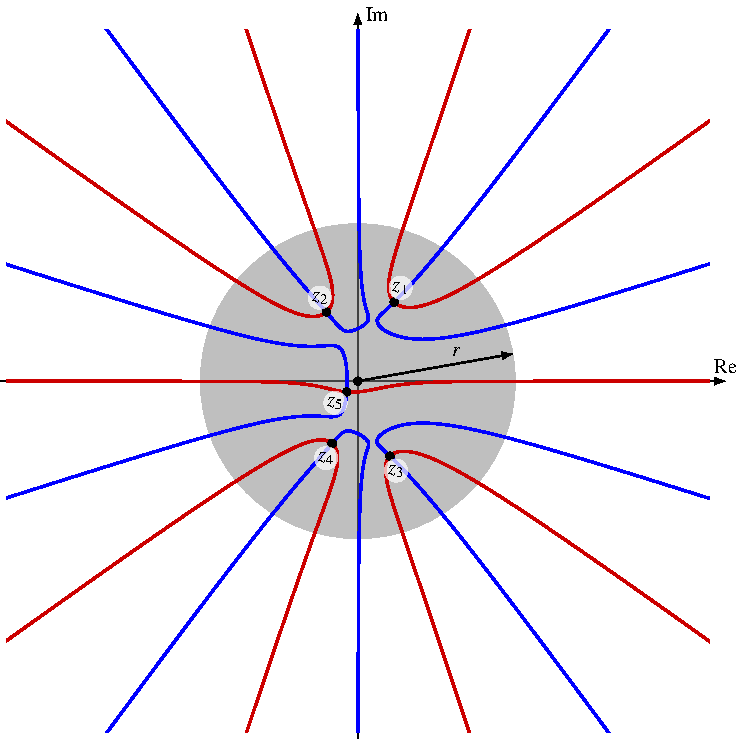
\includegraphics{chapters/010-komplex/images/fundamental.pdf}
\caption{Illustration von Gauss' Idee zum Beweis des Fundamentalsatzes
der Algebra anhand eines Polynoms $p(z)$ vom Grad 5.
Die roten Linien bestehen aus den Punkten $z$, für die der
Imaginärteil $\operatorname{Im} p(z)$ verschwindet.
Auf den blauen Kurven verschwindet der Realteil $\operatorname{Re}p(z)$.
Es kann höchstens 5 rote und blaue Kurven geben.
Ein grosser Kreis um den Nullpunkt schneidet abwechslungsweise rote und
blaue Kurven insgesamt je 10 mal.
Also müssen sich diese Kurven im Inneren des grauen Kreises schneiden.
Die Schnittpunkte sind Nullstellen $z_k$ des Polynoms
\label{buch:komplex:fig:fundamental}}
\end{figure}
%

Dieser Satz wird oft Carl Friedrich Gauss zugeschrieben.
\index{Gauss, Carl Friedrich}%
Sein erster Beweis ging von der folgenden Idee aus.
Sei $p(z)\in \mathbb{C}[z]$ ein normiertes Polynom vom Grad $n$.
Da eine Polynomgleichung höchstens $n$ Lösungen haben kann,
bestehen
\[
I=\{z\in\mathbb{C} \mid p(z) \in \mathbb{R} \}
\qquad\text{und}\qquad
R=\{z\in\mathbb{C} \mid p(z) \in i\mathbb{R} \}
\]
aus höchstens $n$ Kurven (Abbildung~\ref{buch:komplex:fig:fundamental},
blaue Kurven für $I$ und rote Kurven für $R$).
Ausserhalb eines grossen Kreises ist die führende Potenz $z^n$ dominant.
Auf dem Kreis mit Radius $r$ finden wir die Werte
\[
r^n (\cos n\varphi + i \sin n\varphi) + o(r^n),
\]
wobei abwechselnd der Real- bzw.~der Imaginärteil verschwinden.
Der Kreis schneidet also abwechseln eine Kurve von $R$ bzw.~von $I$
je $2n$ mal.
Da es sich jeweils nur um $n$ Kurven handelt, muss es im Inneren des
Kreises Schnittpunkte $z_k$ geben.
In einem Schnittpunkt einer roten und blauen Kurve sind sowohl 
Real- wie auch Imaginärteil $0$, er ist eine Nullstelle.

Die Beweisidee von Gauss hat jedoch eine Lücke: sie appelliert an 
intuitiv einleuchtende topologische Eigenschaften der komplexen
Ebene.
Dass solche Eigenschaften trotz ihrer Anschaulichkeit
nicht unbedingt selbstverständlich sind und einen Beweis erfordern,
wird auch in Kapitel~\ref{chapter:jordan} erläutert.

Der erste korrekte Beweis des Fundamentalsatzes wurde von 1814 von
Jean-Robert Argand publiziert \cite{buch:argand}.
\index{Argand, Jean-Robert}%
Argand war ein Buchhändler und Amateurmathematiker aus Genf,
wo er 1768 geboren wurde.
Er starb 1822 in Paris.
Sein Beweis des Fundamentalsatzes wird in Cauchys \emph{Cours d'analyse}
\index{Cauchy, Augustin-Louis}%
\cite{buch:cauchy} verwendet, der Autor Argand aber nicht erwähnt.

Wir werden den Fundamentalsatz in
Abschnitt~\ref{buch:analytisch:ganz:subsection:fundamentalsatz}
mit analytischen Hilfsmitteln beweisen.
Für die Analysis bedeutet dieser Satz, dass man mit dem Körper
$\mathbb{C}$ den Körper erreicht hat, indem jede Faktorisierungsaufgabe
von Polynome immer gelöst werden kann.
Dies hat zum Beispiel zur Konsquenz, dass sich das Integral
\index{Integral}%
jeder rationalen Funktion mit komplexen Koeffizienten immer
in geschlossener Form lösen lässt, wie
in Abschnitt~\ref{buch:ratint:section:bernoulli} gezeigt wird.
Das bedeutet aber noch nicht, dass das Integrationsproblem damit
gelöst ist, denn das Finden der Nullstellen ist immer noch ein
offenes Problem, welches im Kapitel~\ref{chapter:ratint} im Detail
untersucht wird.


%
% 32-nullstellenq.tex -- Nullstellen von Polynomen über Q
%
% (c) 2026 Prof Dr Andreas Müller
%
\subsection{Nullstellen von Polynomen über $\mathbb{Q}$}
Der Fundamentalsatz der Algebra löst das Problem der Faktorisierung
ein einem einzigen Körper.
Jedes Polynom $p(Z)\in \mathbb{C}[Z]$ lässt sich in Linearfaktoren
zerlegen.
Dies ermöglicht zum Beispiel die Partialbruchzerlegung rationaler
Funktionen und steht damit am Anfang der Lösung des Integrationsproblem
für rationale Funktionen, welches in Kapitel~\ref{chapter:ratint}
gelöst wird.
\index{Partialbruchzerlegung}%
Jede rationale Funktion mit komplexen Koeffizienten hat eine
Stammfunktion, die sich als rationale Funktion und eine Linearkombination
von Logarithmusfunktionen der Form $\log(z-\alpha_i)$ ist, wobei die
$\alpha_i\in\mathbb{C}$ die Nullstellen des Nennerpolynoms sind.

Trotz dem unbestreitbaren Erfolg der komplexen Zahlen bleibt ein
grundlegendes Problem für die Anwendung in der Computeralgebra.
\index{Computeralgebra}%
Nicht jede komplexe Zahl hat eine exakte Darstellung in einem Computersystem.
Da $\mathbb{C}=\mathbb{R}(i)$ eine algebraische Erweiterung der 
überabzählbar unendlichen Menge der reellen Zahlen ist, gibt es
überabzählbar unendlich viele komplexe Zahlen.
In einem Computer kann man aber prinzipiell nur abzählbar unendlich
viele Zahlen exakt darstellen.
Gleitkomma-Arithmetik löst das Problem dadurch, dass reelle Zahlen
\index{Gleitkomma-Arithmetik}%
und damit auch komplexe Zahlen approximiert werden.
Die meisten Zahlen, die in numerischen Rechnungen auftreten, sind
daher nur Approximationen und man kann nicht erwarten, die Nullstellen
eines Polynoms exakt zu bestimmen, selbst bei Polynomen mit
rationalen Koeffizienten, die eine endliche Spezifikation haben.

Ein Computeralgebrasystem möchte entscheiden können, ob eine Gleichung
exakt erfüllt ist.
Dazu ist eine Approximation nicht ausreichen.
Es muss ein Zahlenbereich gefunden werden, in dem solche exakten Aussagen
möglich sind.
Er muss die arithmetische Grundoperationen ermöglichen, d.~h.~er muss
die rationalen Zahlen enthalten.
Die verbreitete freie Softwarebibliothek GMP \cite{buch:gmp} realisiert
\index{GMP}%
die Arithmetik mit rationalen Zahlen mit beliebig grossen Zählern und
Nennern, solange diese im Speicher Platz haben.
Man kann zwar nicht jede rationale Zahl im Computer darstellen, aber
man kann jede Zahl, die man im Laufe einer Berechnung antrifft, exakt
darstellen.

In einem Computeralgebrasystem muss man also nicht für jedes mathematische
Objekt von Anfang an eine exakte Darstellung haben, aber man muss
jedes Objekt, das im Laufe einer Rechnunung auftritt, exakt darstellen
können.
Möchte man eine quadratische Gleichung lösen, braucht es im Allgemeinen
eine Darstellung für jede beliebige Quadratwurzel von rationalen
Zahlen.
Ein Computeralgebrasystem führt dazu neue Symbole mit geeigneten
Rechenregeln ein.
Um mit der Wurzel $\!\sqrt{2}$ rechnen zu können, muss man dem
Computeralgebrasystem ein neues Objekt \texttt{sqrt(2)} hinzufügen,
welches die Eigenschaft $\texttt{sqrt(2)}^2 = 2$ hat.
Diese Konstruktion kann iteriert werden, \text{sqrt(sqrt(2))} ist
ein Objekt welches die algebraischen Eigenschaften einer vierten Wurzel
hat.

Der Fundamentalsatz der Algebra erhält in diesem Zusammenhang eine
neue Rolle.
Er garantiert, dass jedes komplexe Polynome eine Nullstelle hat, die
man bei Bedarf auch numerisch berechnen kann.
Für eine algebraisch exakte Darstellung ist diese numerische Darstellung
aber nicht nötig.
Viel wichtiger es, eine solche Nullstelle als ein Element zu interpretieren,
um das der Körper $\mathbb{Q}$ erweitert werden muss, damit die Rechnung
weitergeführt werden kann.

Die Berechnung in einem Computeralgebrasystem beginnt also mit den rationalen
Zahlen $\mathbb{Q}$.
Jedesmal, wenn eine Wurzel oder eine Nullstelle eines Polynoms auftritt,
wird der Körper der darstellbaren Zahlen um das algebraische Element
$\alpha$ erweitert.
Die weiteren Rechnungen finden im erweiterten Körper $K=\mathbb{Q}(\alpha)$
statt.
Die algebraischen Eigenschaften des Elements $\alpha$ sind Teil der
Spezifikation von $\alpha$.
Auch die imaginäre Einheit ist von dieser Art.

Ein Computeralgebrasystem muss aber auch mit anderen Grössen umgehen
können, zum Beispiel mit der Kreiszahl $\pi$ oder der Basis $e$
\index{Kreiszahl}%
\index{pi@$\pi$}%
\index{e@$e$}%
der natürlichen Logarithmen.
Auch diese Zahlen existieren als Elemente in $\mathbb{C}$.
Für die Rechnung in einem Computeralgebrasystem ist die Darstellung von $\pi$
oder $e$ als Gleitkommazahl nicht ausreichend.
Aber auch diese Zahlen können durch ihre algebraischen Eigenschaften
charakterisiert werden.
Es gibt zwar kein Polynom in $\mathbb{Q}[z]$, das $\pi$ oder $e$ als
Nullstelle hat, da diese Zahlen transzendent sind.
Die Potenzen $\pi^k$, $k\in\mathbb{N}$ sind über $\mathbb{Q}$ linear
unabhängig.
Das bedeutet aber nur, dass man eine Potenz von $\pi$ niemals
durch niedrigere Potenzen wird ausdrücken können, wie das bei den
algebraischen Elementen der Fall ist.
Dafür gibt es Beziehungen wie $e^{i\pi}=-1$, mit denen Exponentialausdrücke
vereinfacht werden können, die $\pi$ im Exponenten enthalten.
Für die praktischen Zwecke eines Computeralgebrasystems genügt dies.
Für jeden im Laufe der Rechnung auftretenden Ausdruck lässt sich eine
Darstellung im Computer finden.

In der Analysis lernt man, dass für die Definition der Ableitung einer
Funktion ein Grenzwert in $\mathbb{R}$ nötig ist.
In Abschnitt~\ref{buch:holomorph:section:holomorph} werden wir zeigen,
wie sich die Ableitung auf komplexe Funktionen ausdehnen lässt.
Auch in diesem Szenario garantieren die analytischen Eigenschaften des
Körpers $\mathbb{C}$, dass die Ableitung als Zahl in $\mathbb{C}$ existiert.
Es ist zwar möglich, Ableitungen numerisch zu berechnen, eine besonders
elegante Methode wird in Kapitel~\ref{chapter:step} beschrieben.
Dies ist aber wieder nicht die Art und Weise, wie ein Computeralgebrasystem
mit der Ableiltung umgeht.
Hierfür werden die algebraischen Eigenschaften des Ableitungsoperators
verwendet, die man als die Ableitungsregeln aus der Analysis kennt.
Sie ermöglichen, die Ableitung beliebig komplizierter Ausdrücke
zu berechnen, sofern man nur die Ableitungsregeln für die Komponenten
des Ausdrucks kennt.
Man muss zum Beispiel nicht wissen, wie man einen Wert von $f(x)=e^{1291x}$
berechnen kann, um die Ableitung zu berechnen.
Die Ableitungsregeln sagen $f'(x)=1291 e^{1291x}$.
Abschnitt~\ref{buch:intalg:section:elementar} wird dies formalisieren.

Auch die Definition des Integrals verwendet die analytische
Vollständigkeit von $\mathbb{C}$.
Die Existenz von Werten eines Integrals ist dadurch gesichert.
Ein Computeralgebrasystem ist jedoch nicht an Werten interessiert,
sondern an algebraischen Ausdrücken für die Stammfunktion.
Um einen solchen zu finden, ist die Definition des Riemann-Integrals
\index{Riemann-Integral}%
\index{Integral, Riemann-}%
als Grenzwert einer Summe von Rechteckflächen nicht zweckmässig.
Die Lösung wird durch den Hauptsatz der Infinitesimalrechnung gegeben.
\index{Hauptsatz}%
Die Stammfunktion ist durch die rein algebraische Eigenschaft
charakterisiert, dass der Ableitungsoperator aus der Stammfunktion
den Integranden produziert.
Auch das Integrationsproblem ist damit auf ein rein algebraisches
Problem reduziert, welches in Kapitel~\ref{chapter:intalg}
studiert wird.














